% Options for packages loaded elsewhere
\PassOptionsToPackage{unicode}{hyperref}
\PassOptionsToPackage{hyphens}{url}
\PassOptionsToPackage{dvipsnames,svgnames,x11names}{xcolor}
%
\documentclass[
  letterpaper,
  DIV=11,
  numbers=noendperiod,
  oneside]{scrreprt}

\usepackage{amsmath,amssymb}
\usepackage{iftex}
\ifPDFTeX
  \usepackage[T1]{fontenc}
  \usepackage[utf8]{inputenc}
  \usepackage{textcomp} % provide euro and other symbols
\else % if luatex or xetex
  \usepackage{unicode-math}
  \defaultfontfeatures{Scale=MatchLowercase}
  \defaultfontfeatures[\rmfamily]{Ligatures=TeX,Scale=1}
\fi
\usepackage{lmodern}
\ifPDFTeX\else  
    % xetex/luatex font selection
\fi
% Use upquote if available, for straight quotes in verbatim environments
\IfFileExists{upquote.sty}{\usepackage{upquote}}{}
\IfFileExists{microtype.sty}{% use microtype if available
  \usepackage[]{microtype}
  \UseMicrotypeSet[protrusion]{basicmath} % disable protrusion for tt fonts
}{}
\makeatletter
\@ifundefined{KOMAClassName}{% if non-KOMA class
  \IfFileExists{parskip.sty}{%
    \usepackage{parskip}
  }{% else
    \setlength{\parindent}{0pt}
    \setlength{\parskip}{6pt plus 2pt minus 1pt}}
}{% if KOMA class
  \KOMAoptions{parskip=half}}
\makeatother
\usepackage{xcolor}
\usepackage[left=1in,marginparwidth=2.0666666666667in,textwidth=4.1333333333333in,marginparsep=0.3in]{geometry}
\setlength{\emergencystretch}{3em} % prevent overfull lines
\setcounter{secnumdepth}{5}
% Make \paragraph and \subparagraph free-standing
\ifx\paragraph\undefined\else
  \let\oldparagraph\paragraph
  \renewcommand{\paragraph}[1]{\oldparagraph{#1}\mbox{}}
\fi
\ifx\subparagraph\undefined\else
  \let\oldsubparagraph\subparagraph
  \renewcommand{\subparagraph}[1]{\oldsubparagraph{#1}\mbox{}}
\fi


\providecommand{\tightlist}{%
  \setlength{\itemsep}{0pt}\setlength{\parskip}{0pt}}\usepackage{longtable,booktabs,array}
\usepackage{calc} % for calculating minipage widths
% Correct order of tables after \paragraph or \subparagraph
\usepackage{etoolbox}
\makeatletter
\patchcmd\longtable{\par}{\if@noskipsec\mbox{}\fi\par}{}{}
\makeatother
% Allow footnotes in longtable head/foot
\IfFileExists{footnotehyper.sty}{\usepackage{footnotehyper}}{\usepackage{footnote}}
\makesavenoteenv{longtable}
\usepackage{graphicx}
\makeatletter
\def\maxwidth{\ifdim\Gin@nat@width>\linewidth\linewidth\else\Gin@nat@width\fi}
\def\maxheight{\ifdim\Gin@nat@height>\textheight\textheight\else\Gin@nat@height\fi}
\makeatother
% Scale images if necessary, so that they will not overflow the page
% margins by default, and it is still possible to overwrite the defaults
% using explicit options in \includegraphics[width, height, ...]{}
\setkeys{Gin}{width=\maxwidth,height=\maxheight,keepaspectratio}
% Set default figure placement to htbp
\makeatletter
\def\fps@figure{htbp}
\makeatother
\newlength{\cslhangindent}
\setlength{\cslhangindent}{1.5em}
\newlength{\csllabelwidth}
\setlength{\csllabelwidth}{3em}
\newlength{\cslentryspacingunit} % times entry-spacing
\setlength{\cslentryspacingunit}{\parskip}
\newenvironment{CSLReferences}[2] % #1 hanging-ident, #2 entry spacing
 {% don't indent paragraphs
  \setlength{\parindent}{0pt}
  % turn on hanging indent if param 1 is 1
  \ifodd #1
  \let\oldpar\par
  \def\par{\hangindent=\cslhangindent\oldpar}
  \fi
  % set entry spacing
  \setlength{\parskip}{#2\cslentryspacingunit}
 }%
 {}
\usepackage{calc}
\newcommand{\CSLBlock}[1]{#1\hfill\break}
\newcommand{\CSLLeftMargin}[1]{\parbox[t]{\csllabelwidth}{#1}}
\newcommand{\CSLRightInline}[1]{\parbox[t]{\linewidth - \csllabelwidth}{#1}\break}
\newcommand{\CSLIndent}[1]{\hspace{\cslhangindent}#1}

\KOMAoption{captions}{tableheading}
\makeatletter
\@ifpackageloaded{tcolorbox}{}{\usepackage[skins,breakable]{tcolorbox}}
\@ifpackageloaded{fontawesome5}{}{\usepackage{fontawesome5}}
\definecolor{quarto-callout-color}{HTML}{909090}
\definecolor{quarto-callout-note-color}{HTML}{0758E5}
\definecolor{quarto-callout-important-color}{HTML}{CC1914}
\definecolor{quarto-callout-warning-color}{HTML}{EB9113}
\definecolor{quarto-callout-tip-color}{HTML}{00A047}
\definecolor{quarto-callout-caution-color}{HTML}{FC5300}
\definecolor{quarto-callout-color-frame}{HTML}{acacac}
\definecolor{quarto-callout-note-color-frame}{HTML}{4582ec}
\definecolor{quarto-callout-important-color-frame}{HTML}{d9534f}
\definecolor{quarto-callout-warning-color-frame}{HTML}{f0ad4e}
\definecolor{quarto-callout-tip-color-frame}{HTML}{02b875}
\definecolor{quarto-callout-caution-color-frame}{HTML}{fd7e14}
\makeatother
\makeatletter
\makeatother
\makeatletter
\@ifpackageloaded{bookmark}{}{\usepackage{bookmark}}
\makeatother
\makeatletter
\@ifpackageloaded{caption}{}{\usepackage{caption}}
\AtBeginDocument{%
\ifdefined\contentsname
  \renewcommand*\contentsname{Table of contents}
\else
  \newcommand\contentsname{Table of contents}
\fi
\ifdefined\listfigurename
  \renewcommand*\listfigurename{List of Figures}
\else
  \newcommand\listfigurename{List of Figures}
\fi
\ifdefined\listtablename
  \renewcommand*\listtablename{List of Tables}
\else
  \newcommand\listtablename{List of Tables}
\fi
\ifdefined\figurename
  \renewcommand*\figurename{Figure}
\else
  \newcommand\figurename{Figure}
\fi
\ifdefined\tablename
  \renewcommand*\tablename{Table}
\else
  \newcommand\tablename{Table}
\fi
}
\@ifpackageloaded{float}{}{\usepackage{float}}
\floatstyle{ruled}
\@ifundefined{c@chapter}{\newfloat{codelisting}{h}{lop}}{\newfloat{codelisting}{h}{lop}[chapter]}
\floatname{codelisting}{Listing}
\newcommand*\listoflistings{\listof{codelisting}{List of Listings}}
\usepackage{amsthm}
\theoremstyle{definition}
\newtheorem{definition}{Definition}[chapter]
\theoremstyle{remark}
\AtBeginDocument{\renewcommand*{\proofname}{Proof}}
\newtheorem*{remark}{Remark}
\newtheorem*{solution}{Solution}
\makeatother
\makeatletter
\@ifpackageloaded{caption}{}{\usepackage{caption}}
\@ifpackageloaded{subcaption}{}{\usepackage{subcaption}}
\makeatother
\makeatletter
\@ifpackageloaded{tcolorbox}{}{\usepackage[skins,breakable]{tcolorbox}}
\makeatother
\makeatletter
\@ifundefined{shadecolor}{\definecolor{shadecolor}{rgb}{.97, .97, .97}}
\makeatother
\makeatletter
\makeatother
\makeatletter
\@ifpackageloaded{sidenotes}{}{\usepackage{sidenotes}}
\@ifpackageloaded{marginnote}{}{\usepackage{marginnote}}
\makeatother
\makeatletter
\makeatother
\makeatletter
\@ifpackageloaded{tcolorbox}{}{\usepackage[many]{tcolorbox}}
\makeatother
%%%% ---foldboxy preamble ----- %%%%%

\definecolor{fbx-default-color1}{HTML}{c7c7d0}
\definecolor{fbx-default-color2}{HTML}{a3a3aa}

\definecolor{fbox-color1}{HTML}{c7c7d0}
\definecolor{fbox-color2}{HTML}{a3a3aa}

% arguments: #1 typelabelnummer: #2 titel: #3
\newenvironment{fbx}[3]{\begin{tcolorbox}[enhanced, breakable,%
attach boxed title to top*={xshift=1.4pt},
boxed title style={boxrule=0.0mm, fuzzy shadow={1pt}{-1pt}{0mm}{0.1mm}{gray}, arc=.3em, rounded corners=east, sharp corners=west}, colframe=#1-color2, colbacktitle=#1-color1, colback = white, coltitle=black,  titlerule=0mm, toprule=0pt, bottomrule=.7pt, leftrule=.3em, rightrule=0pt, outer arc=.3em,  arc=0pt,	 sharp corners = east, left=.5em, bottomtitle=1mm, toptitle=1mm,title=\textbf{#2}\hspace{0.5em}{#3}]}
{\end{tcolorbox}}

% boxed environment with right border
\newenvironment{fbxSimple}[3]{\begin{tcolorbox}[enhanced, breakable,%
attach boxed title to top*={xshift=1.4pt},
boxed title style={boxrule=0.0mm, fuzzy shadow={1pt}{-1pt}{0mm}{0.1mm}{gray}, arc=.3em, rounded corners=east, sharp corners=west}, colframe=#1-color2, colbacktitle=#1-color1, colback = white, coltitle=black,  titlerule=0mm, toprule=0pt, bottomrule=.7pt, leftrule=.3em, rightrule=.7pt, outer arc=.3em,  	left=.5em, right=.5em, bottomtitle=1mm, toptitle=1mm,title=\textbf{#2}\hspace{0.5em}{#3}]}
{\end{tcolorbox}}

%%%% --- end foldboxy preamble ----- %%%%%
%%==== colors from yaml ===%
\definecolor{Theorem-color1}{HTML}{948bde}
\definecolor{Theorem-color2}{HTML}{584eab}
\definecolor{DONE-color1}{HTML}{cce7b1}
\definecolor{DONE-color2}{HTML}{86b754}
\definecolor{Corollary-color1}{HTML}{948bde}
\definecolor{Corollary-color2}{HTML}{584eab}
\definecolor{Conjecture-color1}{HTML}{948bde}
\definecolor{Conjecture-color2}{HTML}{584eab}
\definecolor{Definition-color1}{HTML}{d999d3}
\definecolor{Definition-color2}{HTML}{a01793}
\definecolor{Feature-color1}{HTML}{c0c0c0}
\definecolor{Feature-color2}{HTML}{808080}
\definecolor{TODO-color1}{HTML}{e7b1b4}
\definecolor{TODO-color2}{HTML}{8c3236}
%=============%
\ifLuaTeX
  \usepackage{selnolig}  % disable illegal ligatures
\fi
\IfFileExists{bookmark.sty}{\usepackage{bookmark}}{\usepackage{hyperref}}
\IfFileExists{xurl.sty}{\usepackage{xurl}}{} % add URL line breaks if available
\urlstyle{same} % disable monospaced font for URLs
\hypersetup{
  pdftitle={Introduction aux nombres complexes et polynômes},
  pdfauthor={Jérôme Soucy},
  colorlinks=true,
  linkcolor={blue},
  filecolor={Maroon},
  citecolor={Blue},
  urlcolor={Blue},
  pdfcreator={LaTeX via pandoc}}

\title{Introduction aux nombres complexes et polynômes}
\author{Jérôme Soucy}
\date{2023-07-07}

\begin{document}
\maketitle
\ifdefined\Shaded\renewenvironment{Shaded}{\begin{tcolorbox}[interior hidden, borderline west={3pt}{0pt}{shadecolor}, frame hidden, enhanced, boxrule=0pt, sharp corners, breakable]}{\end{tcolorbox}}\fi

\renewcommand*\contentsname{Table of contents}
{
\hypersetup{linkcolor=}
\setcounter{tocdepth}{2}
\tableofcontents
}
\bookmarksetup{startatroot}

\hypertarget{index}{%
\chapter{Index}\label{index}}

Bonjour!

\bookmarksetup{startatroot}

\hypertarget{arithmuxe9tique-uxe9luxe9mentaire}{%
\chapter{Arithmétique
élémentaire}\label{arithmuxe9tique-uxe9luxe9mentaire}}

\providecommand{\R}{\mathbb{R}}
\providecommand{\Q}{\mathbb{Q}}
\providecommand{\C}{\mathbb{C}}
\newcommand{\N}{\mathbb{N}}
\newcommand{\Z}{\mathbb{Z}}
\newcommand{\zbar}{\overline{z}}
\newcommand{\RE}{\textrm{Re}\,}
\newcommand{\IM}{\textrm{Im}\,}
\newcommand{\Arg}{\textrm{Arg}\,}
\newcommand{\iu}{\textrm{i}}
\newcommand{\boitevide}{\square}

Avant d'introduire les nombres complexes, il serait pertinent de revoir
quelques propriétés de ce que nous avons coutume d'appeler nombre, et de
faire l'inventaire des objets mathématiques qui appartiennent à cette
catégorie.

\hypertarget{les-nombres-en-guxe9nuxe9ral}{%
\section{Les nombres en général}\label{les-nombres-en-guxe9nuxe9ral}}

Les nombres --- qu'on les qualifie de naturels, entiers, rationnels,
réels ou complexes --- sont des objets mathématiques qui une fois
déshabillés des attributs que nous leur prêtons, se réduisent à n'être
que des ensembles. Au moyen d'efforts considérables dans certains cas,
tout nombre \(x\) peut s'écrire de manière à ce que \(x=\{\ldots\}\), où
les trois points sont eux-mêmes des ensembles, des ensembles
d'ensembles, etc. Si ces définitions --- qu'on pourrait qualifier
d'ensemblistes --- des nombres sont d'une importance capitale, tous
conviendront que nos raisonnements quotidiens qui les font intervenir
portent davantage sur leurs caractéristiques que sur leur définition.
Ainsi, en pensant au nombre \(2\), l'image de deux points, semblables à
ceux qu'on retrouve sur un dé à 6 faces, se présentera à notre esprit
plus rapidement que la définition du nombre \(2\) donnée par John von
Neumann (voir Neumann (1923)) voulant que
\(2=\{\emptyset,\{\emptyset\}\}\), où \(\emptyset\) désigne l'ensemble
ne comportant aucun élément (l'ensemble vide).

\hypertarget{deux-opuxe9rations-fondamentales}{%
\section{Deux opérations
fondamentales}\label{deux-opuxe9rations-fondamentales}}

Dès le début du primaire, on apprend à additionner et à multiplier des
nombres. Ils sont d'abord naturels, puis lorsque l'élève termine ses
études primaires, il est réputé en mesure d'effectuer ces opérations
avec des nombres appartenant à des ensembles plus vastes, comme le sont
les entiers et les nombres fractionnaires\footnote{Éventuellement
  appelés nombres rationnels.}. Dans tous les cas, certaines propriétés,
qu'on pourrait qualifier de «~lois de l'arithmétique~», sont vérifiées.
En voici quelques-unes :

\begin{enumerate}
\def\labelenumi{\arabic{enumi}.}
\tightlist
\item
  L'addition et la multiplication sont des opérations associatives~;
\item
  L'addition et la multiplication sont des opérations commutatives~;
\item
  La multiplication est distributive sur l'addition~;
\item
  Un ensemble de nombres \(E\) est stable pour l'addition et la
  multiplication.
\end{enumerate}

Voici ce qu'on entend par ces lois.

\hypertarget{associativituxe9}{%
\section{Associativité}\label{associativituxe9}}

Le fait qu'écrire \(1+2+5\) ne pose aucune ambiguïté découle du fait que
l'opération d'addition soit associative. Qu'on calcule \((1+2)+5\) ou
\(1+(2+5)\), le résultat sera le même. De la même manière,
\[3\times 4\times 5=3\times (4\times 5)=(3\times 4)\times 5.\]
L'associativité c'est la possibilité de déplacer une paire de
parenthèses sans modifier le résultat. Bien que l'addition et la
multiplication soient des opérations associatives, le déplacement de
parenthèses n'est pas forcément valable si ces deux opérations sont
présentes dans un même calcul. Par exemple, pour calculer
\(1+2\times 5\), on ne peut pas calculer n'importe quelle des deux
expressions \((1+2)\times 5\) et \(1+(2\times 5)\). On \emph{convient}
que l'expression \(1+2\times 5\) correspond à \(1+(2\times 5)\). Il
s'agit ainsi d'une convention d'écriture plutôt que d'un résultat
mathématique. On réfère souvent à cette convention en invoquant la
priorité des opérations. Encore une fois, ce sont des expressions qui ne
font que traduire l'économie de parenthèses qu'il nous est possible de
réaliser ; plutôt que d'écrire
\[1+((2\times 7)+(3\times 3-(8\times 2))),\] on convient d'écrire
simplement \(1+2\times 7+3\times 3-8\times 2\). Notons que ce ne sont
pas toutes les opérations qui sont associatives. Par exemple,
\[(3\div 4)\div 5\neq 3\div(4\div 5).\] Le membre de gauche correspond à
la fraction \(\frac{3}{20}\) alors que le membre de droite à
\(\frac{15}{4}\). Il s'agit là de deux fractions qui ne sont pas
équivalentes.

L'idée d'associativité s'étend au-delà des opérations sur les nombres.
Par exemple, si \(f,g\) et \(h\) sont des fonctions, alors
\((f\circ g)\circ h=f\circ (g\circ h)\). À titre d'exemple, posons
\(f(x)=x^2, g(x)=\sin(x)\) et \(h(x)=x+1\). Nous avons que
\((f\circ g)(x)=\sin^2(x)\), d'où
\[\left((f\circ g)\circ h\right)(x)=\sin^2(h(x))=\sin^2(x+1).\] De même,
\((g\circ h)(x)=\sin(x+1)\), d'où
\[\left(f\circ (g\circ h)\right)(x)=f(\sin(x+1))=(\sin(x+1))^2=\sin^2(x+1).\]
Encore une fois, l'égalité \((\sin (x+1))^2=\sin^2(x+1)\) est vraie
puisqu'il s'agit d'une convention d'écriture.

\hypertarget{commutativituxe9}{%
\section{Commutativité}\label{commutativituxe9}}

Si l'associativité est la possibilité de déplacer des parenthèses, la
commutativité est, pour sa part, la possibilité d'inverser l'ordre des
deux arguments intervenant dans l'opération. Par exemple, l'équation
\[1+3=3+1\] est vraie, puisque l'addition est une opération commutative.
La multiplication de nombres est aussi une opération
commutative\footnote{Il est possible de définir une opération de
  multiplication sur certains ensembles de nombres, de telle sorte que
  la multiplication ne soit pas commutative. C'est notamment le cas avec
  l'ensemble des quaternions. Comme ces nombres sont l'apanage des
  mathématiques avancées et de la physique théorique, nous ne nous
  étendrons pas plus loin sur le sujet.}. Il en va autrement de la
multiplication matricielle. Par exemple, si
\[A=\begin{pmatrix} 0 &1 \\ 2 & 3\\ \end{pmatrix}\qquad\text{et}\qquad B=\begin{pmatrix} 1 &-1 \\ 0 & 2\\\end{pmatrix},\]
alors
\[AB=\begin{pmatrix} 0 &2 \\ 2 & 4\\ \end{pmatrix}\qquad\text{et}\qquad BA=\begin{pmatrix} -2 &-2 \\ 4 & 6\\\end{pmatrix}.\]

Un énoncé du type «~la multiplication est commutative~» doit donc être
mis en contexte~; il faut bien comprendre de quelle multiplication il
s'agit. En principe, on doit toujours préciser l'ensemble sur lequel
l'opération est définie. Il serait plus juste de dire que «~la
multiplication définie sur l'ensemble des nombres réels est une
opération commutative~» alors que «~la multiplication définie sur
l'ensemble des matrices \(2\times 2\) n'est pas une opération
commutative~». L'algèbre moderne s'efforce de clarifier ces notions en
introduisant ce qu'on appelle des \emph{structures algébriques}.

\hypertarget{distributivituxe9-de-la-multiplication-par-rapport-uxe0-laddition}{%
\section{Distributivité de la multiplication par rapport à
l'addition}\label{distributivituxe9-de-la-multiplication-par-rapport-uxe0-laddition}}

On l'a vu, dans une même expression, il est possible d'y voir deux
opérations de nature différente. Un cas important est celui d'une
expression où sont présentes l'addition et la multiplication. C'est ce
qu'on constate dans l'expression \(5\times(1+3)\). Pour l'évaluer, on
peut bien sûr évaluer la somme entre parenthèses, puis multiplier \(5\)
par \(4\). Une autre avenue possible est de «~distribuer~» la
multiplication par rapport à l'addition, ce qui signifie calculer
\((5\times 1)+(5\times 3)\). Lorsqu'on affirme que la multiplication est
distributive par rapport à l'addition, cela signifie que pour tous
nombres \(a,b\) et \(c\), on a \[a\times (b+c)=a\times b+a\times c.\]

\hypertarget{stabilituxe9-dun-ensemble-par-rapport-uxe0-une-opuxe9ration}{%
\section{Stabilité d'un ensemble par rapport à une
opération}\label{stabilituxe9-dun-ensemble-par-rapport-uxe0-une-opuxe9ration}}

\marginnote{\begin{footnotesize}

\begin{tcolorbox}[enhanced jigsaw, titlerule=0mm, colback=white, leftrule=.75mm, colframe=quarto-callout-note-color-frame, left=2mm, opacityback=0, toprule=.15mm, bottomrule=.15mm, breakable, title=\textcolor{quarto-callout-note-color}{\faInfo}\hspace{0.5em}{Note}, coltitle=black, rightrule=.15mm, opacitybacktitle=0.6, bottomtitle=1mm, toptitle=1mm, arc=.35mm, colbacktitle=quarto-callout-note-color!10!white]

Le symbole \(\Z\), utilisé pour représenter l'ensemble des entiers, est
la première lettre du mot allemand zahl qui signifie «~nombre~».

\end{tcolorbox}

\end{footnotesize}}

Étant donnés des nombres \(a\) et \(b\) appartenant à un ensemble de
nombres \(E\), leur somme et leur produit appartiennent toujours à
l'ensemble \(E\). Ce n'est pas toujours le cas pour le résultat d'une
opération. À titre d'exemple, l'ensemble des nombres naturels n'est pas
stable pour la soustraction. En effet, ce ne sont pas tous les problèmes
de soustraction\footnote{Un problème de soustraction consiste à trouver
  une solution à une équation de type \(a+\boitevide=b\).} qui admettent
une solution; c'est notamment le cas du problème \(5+\boitevide=3\).
L'ensemble des entiers règle le problème de la stabilité pour
l'opération de la soustraction de nombres naturels, mais cela n'améliore
guère les choses pour les problèmes de division.

Prenons deux nombres naturels \(a\) et \(b\), tels que \(b\) soit non
nul, et considérons l'équation \(b\times \boitevide = a\). Il arrive que
cette équation possède une solution qui est dans \(\N\), mais ce n'est
généralement pas le cas. Par exemple, \(3\times \boitevide = 12\)
possède une solution ---~le nombre \(4\)~---, mais l'équation
\(3\times \boitevide = 13\) n'en possède pas.

\marginnote{\begin{footnotesize}

\begin{tcolorbox}[enhanced jigsaw, titlerule=0mm, colback=white, leftrule=.75mm, colframe=quarto-callout-note-color-frame, left=2mm, opacityback=0, toprule=.15mm, bottomrule=.15mm, breakable, title=\textcolor{quarto-callout-note-color}{\faInfo}\hspace{0.5em}{Note}, coltitle=black, rightrule=.15mm, opacitybacktitle=0.6, bottomtitle=1mm, toptitle=1mm, arc=.35mm, colbacktitle=quarto-callout-note-color!10!white]

L'ensemble des fractions, aussi appelé ensemble des nombres rationnels,
est représenté par le symbole \(\mathbb{Q}\).

L'ensemble des nombres réels est représenté par le symbole \(\R\).

\end{tcolorbox}

\end{footnotesize}}

L'ajout des nombres fractionnaires permet non seulement de résoudre ce
problème dans le cas où \(a\) et \(b\) sont des nombres naturels,
\emph{mais aussi de le faire dans le cas où \(a\) et \(b\) sont des
nombres fractionnaires}. C'est cette propriété qu'on évoque lorsqu'on
mentionne que les nombres fractionnaires sont stables pour l'opération
de division.

Vers le 5ᵉ siècle avant notre ère, les mathématiciens grecs ont tenté de
mesurer la longueur de l'hypoténuse d'un triangle rectangle dont les
côtés adjacents à l'angle droit sont de longueur \(1\). En utilisant le
théorème de Pythagore, ils ont ramené le problème à celui de trouver un
nombre \(x\) tel que \(2=x^2\). Ils en sont venus à la conclusion que
\(x\) ne pouvait être le quotient de deux nombres entiers. Bien sûr, le
langage utilisé pour exprimer cette constatation était fort différent.
On parlait plutôt d'une quantité \emph{incommensurable}, ou encore
\emph{inexprimable}. Le tout rédigé en grec ancien! On ignore toujours
si le problème du calcul de la mesure de l'hypoténuse d'un triangle
rectangle est le premier qui a amené les Grecs à considérer des nombres
irrationnels. Cette découverte suggère néanmoins de définir un ensemble
de nombres plus vaste, comprenant le nombre \(\sqrt{2}\), mais aussi
tous les «~trous~» sur la droite numérique entre les nombres rationnels.
Pour plus d'information sur le nombre \(\sqrt{2}\) et l'extraction des
racines carrées, voir Rittaud (2006). L'existence de tels nombres
signifiait que les fractions ne remplissaient pas complètement la droite
numérique, qu'on associe à l'ensemble des nombres réels.

\bookmarksetup{startatroot}

\hypertarget{duxe9finition-des-nombres-complexes}{%
\chapter{Définition des nombres
complexes}\label{duxe9finition-des-nombres-complexes}}

\providecommand{\R}{\mathbb{R}}
\providecommand{\Q}{\mathbb{Q}}
\providecommand{\C}{\mathbb{C}}
\newcommand{\N}{\mathbb{N}}
\newcommand{\Z}{\mathbb{Z}}
\newcommand{\zbar}{\overline{z}}
\newcommand{\RE}{\textrm{Re}\,}
\newcommand{\IM}{\textrm{Im}\,}
\newcommand{\Arg}{\textrm{Arg}\,}
\newcommand{\iu}{\textrm{i}}
\newcommand{\boitevide}{\square}

\leavevmode\vadjust pre{\hypertarget{Definition-3.1}{}}%
\begin{fbxSimple}{Definition}{Definition 3.1}{}
\phantomsection\label{Definition-3.1}
On appelle \textbf{unité imaginaire} un nombre qui, multiplié par
lui-même, vaut \(-1\). On le notera \(\iu\).

\end{fbxSimple}

\marginnote{\begin{footnotesize}

\begin{tcolorbox}[enhanced jigsaw, titlerule=0mm, colback=white, leftrule=.75mm, colframe=quarto-callout-note-color-frame, left=2mm, opacityback=0, toprule=.15mm, bottomrule=.15mm, breakable, title=\textcolor{quarto-callout-note-color}{\faInfo}\hspace{0.5em}{Note}, coltitle=black, rightrule=.15mm, opacitybacktitle=0.6, bottomtitle=1mm, toptitle=1mm, arc=.35mm, colbacktitle=quarto-callout-note-color!10!white]

En sciences physiques, plus particulièrement dans le domaine du génie
électrique, le symbole \(\textrm{j}\) est utilisé pour représenter
l'unité imaginaire. Cela est pour éviter toute confusion possible avec
l'intensité d'un courant électrique, qui est souvent représentée par la
lettre \(\iu\).

\end{tcolorbox}

\end{footnotesize}}

Plusieurs commentaires s'imposent après une telle définition. D'abord,
elle se place en opposition avec un fait relayé depuis le secondaire :
un nombre, multiplié par lui-même, ne peut donner une quantité
strictement inférieure à \(0\). Cela s'observe notamment en regardant le
graphe de la fonction \(f(x)=x^2\). Votre étonnement face à cette
nouvelle définition est légitime ; on pourrait le comparer à celui vécu
par les Grecs lorsqu'ils ont été obligés d'admettre que la longueur de
l'hypoténuse d'un triangle rectangle dont les deux cathètes mesurent une
unité n'était pas un nombre, en vertu du sens attribué à ce concept.

L'arrivée de cet objet mathématique dans le cercle des nombres ne doit
pas perturber les lois de l'arithmétique ; sommes et produits faisant
intervenir ce nouvel arrivant doivent être bien définis. Si \(a\) et
\(b\) sont des nombres réels, alors \(b\iu\) doit être un nombre (le
produit de deux nombres est un nombre), tout comme \(a+b\iu\) (la somme
de deux nombres est un nombre). Cela nous conduit à la
\textbf{?@def-nbcomplexe}.

\leavevmode\vadjust pre{\hypertarget{Definition-3.2}{}}%
\begin{fbxSimple}{Definition}{Definition 3.2}{}
\phantomsection\label{Definition-3.2}
On appelle \textbf{nombre complexe} un nombre de la forme \(a+b\,\iu\),
où \(a,b\in\R,\) et \(\iu^2=-1\). On notera \(\C\) l'ensemble des
nombres complexes.

\end{fbxSimple}

Il n'y a plus de place sur la droite numérique pour ces nombres,
contrairement aux éléments des ensembles \(\N,\Z,\Q\) et \(\R\). Puisque
deux nombres réels sont nécessaires pour définir un nombre complexe, il
est naturel d'associer à chaque nombre complexe un couple de nombres
réels, et de les représenter dans un plan. Il convient alors de définir
l'égalité de deux nombres complexes de la manière suivante :

\leavevmode\vadjust pre{\hypertarget{Definition-3.3}{}}%
\begin{fbxSimple}{Definition}{Definition 3.3}{}
\phantomsection\label{Definition-3.3}
Deux nombres complexes \(z=a+b\,\iu\) et \(w=c+d\,\iu\) (où
\(a,b,c,d\in\R\)) \textbf{sont égaux} si \(a=c\) et \(b=d\).

\end{fbxSimple}

\begin{marginfigure}

{\centering 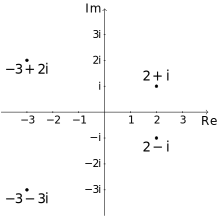
\includegraphics[width=3.125in,height=\textheight]{index_files/mediabag/images/plancomplexe/plancomplexe.pdf}

}

\caption{\label{fig-PlanComplexe}PlanComplexe}

\end{marginfigure}

Plan complexe, aussi appelé plan de Gauss ou encore plan d'Argand.
Quelques points du plan complexe ont été identifiés, et on a précisé
pour chacun de ces points le nombre complexe qui lui est associé.

\hypertarget{somme-de-deux-nombres-complexes}{%
\section{Somme de deux nombres
complexes}\label{somme-de-deux-nombres-complexes}}

Un nombre complexe est défini à partir de deux nombres réels et de
l'unité imaginaire. Lorsqu'on veut faire référence à un nombre complexe,
il n'est pas nécessaire de le nommer à partir des éléments qui le
définissent. Par exemple, on peut dire: \emph{Soit \(z\) un nombre
complexe}. De cela il faut comprendre qu'on peut trouver deux nombres
réels \(a\) et \(b\) tels que \(z=a+b\,\iu\). Cela étant dit, étant
donné deux nombres complexes, comment la somme de ceux-ci peut-elle être
définie afin que les lois de l'arithmétique soient valides? En
s'inspirant de l'opération d'addition des vecteurs, nous pouvons
\emph{définir} l'addition de nombres complexes.

\leavevmode\vadjust pre{\hypertarget{Definition-3.4}{}}%
\begin{fbxSimple}{Definition}{Definition 3.4}{}
\phantomsection\label{Definition-3.4}
Soient \(z_1\) et \(z_2\) deux nombres complexes tels que
\(z_1=x_1+\iu y_1\) et \(z_2=x_2+\iu y_2\), où \(x_1,x_2,y_1\) et
\(y_2\) sont des nombres réels. La \textbf{somme} de \(z_1\) et \(z_2\),
notée \(z_1+z_2\), est le nombre complexe défini par
\[z_1+z_2=x_1+x_2+(y_1+y_2)\iu.\]

\end{fbxSimple}

\begin{tcolorbox}[enhanced jigsaw, titlerule=0mm, colback=white, leftrule=.75mm, colframe=quarto-callout-note-color-frame, left=2mm, opacityback=0, toprule=.15mm, bottomrule=.15mm, breakable, title={Exemple}, coltitle=black, rightrule=.15mm, opacitybacktitle=0.6, bottomtitle=1mm, toptitle=1mm, arc=.35mm, colbacktitle=quarto-callout-note-color!10!white]

La somme des nombres \(1+5\iu\) et \(2-3\iu\) sera \(3+2\iu\).

\end{tcolorbox}

De la même manière, la \textbf{différence} entre \(z_1\) et \(z_2\),
notée \(z_1-z_2\), est le nombre complexe défini par
\[z_1-z_2=x_1-x_2+(y_1-y_2)\iu.\]

\begin{tcolorbox}[enhanced jigsaw, titlerule=0mm, colback=white, leftrule=.75mm, colframe=quarto-callout-note-color-frame, left=2mm, opacityback=0, toprule=.15mm, bottomrule=.15mm, breakable, title={Exemple}, coltitle=black, rightrule=.15mm, opacitybacktitle=0.6, bottomtitle=1mm, toptitle=1mm, arc=.35mm, colbacktitle=quarto-callout-note-color!10!white]

Si \(z_1=1+5\iu\) et \(z_2=2-3\iu\), alors \(z_1-z_2=-1+8\iu\).

\end{tcolorbox}

\begin{marginfigure}

{\centering \includegraphics[width=2.08333in,height=\textheight]{images/timbre.jpg}

}

\caption{\label{fig-timbre}\textbf{?(caption)}}

\end{marginfigure}

Timbre allemand émis en 1977 pour souligner le 200ᵉ anniversaire de
naissance de Carl F. Gauss.

On constate que l'opération d'addition est commutative. En effet, cela
est une conséquence de la commutativité de l'opération d'addition
définie sur les nombres réels~: on a bien que \(x_1+x_2=x_2+x_1\), quels
que soient les nombres réels \(x_1\) et \(x_2\). De la même manière,
l'associativité de l'addition des nombres réels implique l'associativité
de l'addition des nombres complexes. Ainsi,
\[z_1+(z_2+z_3)=(z_1+z_2)+z_3\quad\forall z_1,z_2,z_3\in\C.\] On peut
donc parler de la somme de trois nombres complexes en toute impunité et
la noter \(z_1+z_2+z_3\). Comme c'est aussi le cas dans l'ensemble des
nombres réels, l'opération de soustraction n'est ni associative ni
commutative. On ne doit pas s'étonner de ça~ l'ensemble des nombres
complexes contient l'ensemble des nombres réels.

\hypertarget{parties-ruxe9elle-et-imaginaire}{%
\section{Parties réelle et
imaginaire}\label{parties-ruxe9elle-et-imaginaire}}

Un nombre complexe est entièrement déterminé par un couple de nombres
réels. Réciproquement, un couple de nombre réels détermine un unique
nombre complexe. Il y a donc une bijection entre les éléments de
\(\R^2\) et ceux de \(\C\).

\leavevmode\vadjust pre{\hypertarget{Definition-3.5}{}}%
\begin{fbxSimple}{Definition}{Definition 3.5}{}
\phantomsection\label{Definition-3.5}
Soit \(a,b\in\R\) et soit \(z=a+b\,\iu\) un nombre complexe. On dit
alors que \(a+b\,\iu\) est la forme cartésienne de \(z\). De plus, le
nombre réel \(a\) s'appelle la \textbf{partie réelle} de \(z\), et le
nombre réel \(b\) s'appelle la \textbf{partie imaginaire} de \(z\). On
les note \(\RE(z)\) et \(\IM(z)\) respectivement.

\end{fbxSimple}

\leavevmode\vadjust pre{\hypertarget{todo}{}}%
\begin{fbxSimple}{Theorem}{Theorem 3.6: }{TODO}
\phantomsection\label{todo}
here is some exemplary text

\end{fbxSimple}

\begin{tcolorbox}[enhanced jigsaw, titlerule=0mm, colback=white, leftrule=.75mm, colframe=quarto-callout-warning-color-frame, left=2mm, opacityback=0, toprule=.15mm, bottomrule=.15mm, breakable, title={Remarques}, coltitle=black, rightrule=.15mm, opacitybacktitle=0.6, bottomtitle=1mm, toptitle=1mm, arc=.35mm, colbacktitle=quarto-callout-warning-color!10!white]

\begin{itemize}
\tightlist
\item
  Étant donné un point \((x,y)\) dans le plan, le nombre complexe
  \(x+y\iu\) s'appelle \textbf{l'affixe} du point \((x,y)\).
\item
  Si un nombre complexe peut s'écrire comme \(b\iu\), où \(b\in\R\), on
  dit qu'il est un nombre complexe \textbf{imaginaire pur}, ou encore
  \textbf{purement imaginaire}.
\item
  Lorsqu'on dit d'un nombre qu'il est \textbf{imaginaire}, cela
  sous-entend que l'on considère un nombre complexe dont la partie
  imaginaire est non nulle.
\item
  Au lieu d'écrire \(1\iu\) et \(-1\iu\), on écrit \(\iu\) et \(-\iu\)
  respectivement.
\end{itemize}

\end{tcolorbox}

\marginnote{\begin{footnotesize}

\begin{tcolorbox}[enhanced jigsaw, titlerule=0mm, colback=white, leftrule=.75mm, colframe=quarto-callout-warning-color-frame, left=2mm, opacityback=0, toprule=.15mm, bottomrule=.15mm, breakable, title=\textcolor{quarto-callout-warning-color}{\faExclamationTriangle}\hspace{0.5em}{Warning}, coltitle=black, rightrule=.15mm, opacitybacktitle=0.6, bottomtitle=1mm, toptitle=1mm, arc=.35mm, colbacktitle=quarto-callout-warning-color!10!white]

La partie imaginaire d'un nombre complexe est toujours un nombre réel.

\end{tcolorbox}

\end{footnotesize}}

\hypertarget{produit-de-deux-nombres-complexes}{%
\subsection{Produit de deux nombres
complexes}\label{produit-de-deux-nombres-complexes}}

Considérons deux nombres complexes \(a+b\iu\) et \(c+d\iu\). Le produit
de ces deux nombres reste à définir. Contrairement à l'addition de
vecteurs, qui permet de définir la somme de nombres complexes de manière
analogue, l'algèbre linéaire élémentaire ne nous fournie pas de
multiplication vectorielle qui associe un vecteur du plan à deux
vecteurs du plan. En effet, le produit scalaire de deux vecteurs a pour
résultat un nombre réel, alors que le produit vectoriel de deux vecteurs
donne un vecteur qui est perpendiculaire au plan engendré par les deux
vecteurs dont on calcule le produit. Pour définir l'opération de
multiplication de deux nombres complexes, nous allons appliquer
certaines propriétés que nous aimerions voir vérifiées lorsqu'une
multiplication est effectuée: \begin{align*}
 (a+b\iu)(c+d\iu)&=(a+b\iu)c+(a+b\iu)d\iu&\text{(Distributivité)}\\
 &=ac+(b\iu)c+a(d\iu)+b\iu(d\iu)&\text{(Distributivité)}\\
 &=ac+(b\iu)c+(ad)\iu+b(\iu d)\iu&\text{(Associativité de la $\times$)}\\
 &=ac+c(b\iu)+ad\iu+b(d\iu)\iu&\text{(Commutativité de la $\times$)}\\
  &=ac+(cb)\iu+ad\iu+(bd)\iu\iu&\text{(Associativité de la $\times$)}\\
 &=ac+(bc)\iu+ad\iu+(bd)\iu\iu&\text{(Commutativité de la $\times$)}\\
 &=ac+bc\iu+ad\iu+bd\iu^2&\text{(Convention d'écriture)}\\
 &=ac+bc\iu+ad\iu+bd(-1)&\text{(Définition de $\iu^2$)}\\
 &=ac+bc\iu+ad\iu+(-1)bd&\text{(Commutativité de la $\times$)}\\
 &=ac+(-1)bd+bc\iu+ad\iu&\text{(Commutativité de l'$+$)}\\
 &=ac-bd+(bc+ad)\iu&\text{(Distributivité)}\\
 &=ac-bd+(ad+bc)\iu.&\text{(Commutativité de l'$+$)}
 \end{align*} Ce calcul motive la définition ci-dessous :

\begin{definition}[]\protect\hypertarget{def-produit}{}\label{def-produit}

Soit \(a,b,c\) et \(d\) des nombres réels. Le \textbf{produit des
nombres complexes} \(a+b\iu\) et \(c+d\iu\) est défini comme étant le
nombre \(ac-bd +(ad+bc)\iu\).

\end{definition}

Si on avait fait cette définition \emph{a priori}, elle aurait pu
sembler artificielle. Cependant, le travail effectué précédemment nous
suggère que c'est la manière la plus convenable de définir le produit,
si on souhaite que les lois de l'arithmétique soient vérifiées. On peut
bien sûr le faire \emph{a posteriori}: on montre que l'opération définie
à la Definition~\ref{def-produit} est commutative, associative et
distributive par rapport à l'addition.

\marginnote{\begin{footnotesize}

\begin{tcolorbox}[enhanced jigsaw, titlerule=0mm, colback=white, leftrule=.75mm, colframe=quarto-callout-note-color-frame, left=2mm, opacityback=0, toprule=.15mm, bottomrule=.15mm, breakable, title=\textcolor{quarto-callout-note-color}{\faInfo}\hspace{0.5em}{Note}, coltitle=black, rightrule=.15mm, opacitybacktitle=0.6, bottomtitle=1mm, toptitle=1mm, arc=.35mm, colbacktitle=quarto-callout-note-color!10!white]

Pour multiplier deux nombres complexes, disons \(a+b\iu\) et \(c+d\iu\),
il suffit de retenir que les propriétés d'associativité, de
commutativité et de distributivité sont applicables. En utilisant bien
sûr le fait que \(\iu^2=-1\), on peut facilement calculer leur produit.

\end{tcolorbox}

\end{footnotesize}}

On peut interpréter géométriquement le produit de deux nombres
complexes, mais cela sera grandement facilité par l'introduction de
l'argument d'un nombre complexe que nous aborderons sous peu.

Pour effectuer des calculs faisant intervenir les nombres complexes, il
n'est pas nécessaire de retenir cette définition, mais seulement de
savoir qu'on peut appliquer les propriétés d'associativité, de
commutativité et de distributivité telles que présentées précédemment.
Bien sûr, tôt ou tard, il faudra utiliser le fait que \(\iu^2=-1\) pour
ramener notre expression sous la forme \(a+b\iu\), avec \(a,b\in\R\).

\begin{tcolorbox}[enhanced jigsaw, titlerule=0mm, colback=white, leftrule=.75mm, colframe=quarto-callout-note-color-frame, left=2mm, opacityback=0, toprule=.15mm, bottomrule=.15mm, breakable, title={Exemple}, coltitle=black, rightrule=.15mm, opacitybacktitle=0.6, bottomtitle=1mm, toptitle=1mm, arc=.35mm, colbacktitle=quarto-callout-note-color!10!white]

Trouvez la forme cartésienne du nombre \((1-2\iu)\cdot(-3+4\iu)\).

Nous avons que \begin{align*}
  (1-2\iu)\cdot(-3+4\iu)&=1\cdot(-3+4\iu)-2\iu\cdot(-3+4\iu)\\
  &=-3+4\iu-2\iu\cdot(-3)-2\iu\cdot 4\iu\\
  &=-3+4\iu+6\iu-8\iu^2\\
  &=-3+10\iu-8(-1)\\
  &=-3+10\iu+8\\
  &=5+10\iu.
\end{align*}

\end{tcolorbox}

Soit \(z,w\in\C\), et soient \(\lambda,\mu\in\R\). Alors
\[\RE(\lambda z+\mu w)=\lambda\RE(z)+\mu\RE(w)\quad\text{et}\quad\IM(\lambda z+\mu w)=\lambda\IM(z)+\mu\IM(w).\]

\begin{proof}

Supposons que \(z=a+b\iu\) et \(w=c+d\iu\), où \(a,b,c\) et \(d\in\R\).
Nous avons que
\[\lambda z+\mu w=\lambda(a+b\iu)+\mu(c+d\iu)=\lambda a+\mu c+(\lambda b+\mu d)\iu.\]
Ainsi, \begin{align*}
    \RE(\lambda z+\mu w)&=\lambda a+\mu c=\lambda\RE(z)+\mu\RE(w),\\
    \IM(\lambda z+\mu w)&=\lambda b+\mu d=\lambda\IM(z)+\mu\IM(w).
    \end{align*}

\end{proof}

\marginnote{\begin{footnotesize}

\begin{tcolorbox}[enhanced jigsaw, titlerule=0mm, colback=white, leftrule=.75mm, colframe=quarto-callout-note-color-frame, left=2mm, opacityback=0, toprule=.15mm, bottomrule=.15mm, breakable, title=\textcolor{quarto-callout-note-color}{\faInfo}\hspace{0.5em}{Note}, coltitle=black, rightrule=.15mm, opacitybacktitle=0.6, bottomtitle=1mm, toptitle=1mm, arc=.35mm, colbacktitle=quarto-callout-note-color!10!white]

La partie réelle d'une somme de nombres complexes et la somme des
parties réelles des nombres complexes additionnés.

\end{tcolorbox}

\end{footnotesize}}

Un cas particulier de la proposition précédente est que la partie réelle
d'une somme de nombres complexes est la somme des parties réelles des
nombres complexes additionnés. On peut tirer le même constat dans le cas
de la partie imaginaire. Cependant, la partie réelle du produit de deux
nombres complexes n'est pas le produit des parties réelles des nombres
complexes multipliés.

\marginnote{\begin{footnotesize}

\begin{tcolorbox}[enhanced jigsaw, titlerule=0mm, colback=white, leftrule=.75mm, colframe=quarto-callout-warning-color-frame, left=2mm, opacityback=0, toprule=.15mm, bottomrule=.15mm, breakable, title=\textcolor{quarto-callout-warning-color}{\faExclamationTriangle}\hspace{0.5em}{Warning}, coltitle=black, rightrule=.15mm, opacitybacktitle=0.6, bottomtitle=1mm, toptitle=1mm, arc=.35mm, colbacktitle=quarto-callout-warning-color!10!white]

Il est faux de dire que que la partie réelle du produit de deux nombres
complexes est égale au produit des parties réelles des deux nombres
multipliés. De même, \[\IM(zw)\neq\IM(z)\IM(w)\] en général.

\end{tcolorbox}

\end{footnotesize}}

\hypertarget{inverse}{%
\subsection{Inverse}\label{inverse}}

La définition du produit de deux nombres complexes nous permet de se
questionner sur l'existence de l'inverse (multiplicatif) d'un nombre
complexe. D'abord, l'inverse d'un nombre complexe \(z\) est un nombre
complexe \(w\) tel que \(z\times w=1\). L'inverse de \(z\) est noté
\(\frac{1}{z}\) ou \(z^{-1}\). Cette définition n'a de sens que si
\(z\neq 0\), car dans le cas contraire, il nous faudrait trouver un
\(w\in\C\) tel que \(0\times w=1\), ce qui est bien sûr impossible. On
peut donc supposer que \(z=a+b\iu\), avec \(a,b\in\R\), pas tous les
deux nuls, puis partir à la recherche d'un nombre complexe \(w\) de la
forme \(x+y\iu\), où \(x,y\in\R\). En utilisant la formule donnant le
produit de deux nombres complexes, on doit avoir que
\[\underbrace{ax-by +(ay+bx)\iu}_{zw}=1.\] En égalant parties réelles et
imaginaires (c'est ce qu'on doit faire en vertu de la définition
d'égalité de deux nombres complexes présentée à la
\textbf{?@def-egalite}), nous obtenons les équations \begin{align}
ax-by&=1,\\
ay+bx&=0.
\end{align}

En multipliant la première équation par \(a\) et la seconde par \(b\),
nous obtenons les équations \begin{align}
a^2x-aby&=a,\label{eqn:reelle2}\\
aby+b^2x&=0.\label{eqn:imaginaire2}
\end{align} En additionnant ces équations, on obtient l'équation
\(a^2x+b^2x=a\). Puisque \(a^2+b^2\neq 0,\) (conséquence du fait que
\(a\) et \(b\) ne sont pas tous les deux nuls, qui à son tour découle de
l'observation que \(z\neq 0\)), on est en droit de diviser par
\(a^2+b^2\), et on trouve que \(x=\frac{a}{a^2+b^2}\). En procédant
d'une manière semblable, on trouve que \(y=-\frac{b}{a^2+b^2}\). Ainsi,
l'inverse multiplicatif du nombre complexe \(z=a+b\iu\) est le nombre
complexe \[\frac{a}{a^2+b^2}-\frac{b}{a^2+b^2}\iu.\] Il n'est pas
nécessaire de mémoriser cette formule pour obtenir l'inverse d'un nombre
complexe. Il suffit de multiplier le numérateur et le dénominateur par
une quantité bien choisie. Avant de dévoiler cette quantité, rappelons
d'abord ce qu'on peut faire pour rationaliser le dénominateur du nombre
\(\frac{1}{3+\sqrt{2}}\). On voit au secondaire qu'il suffit de
multiplier le numérateur et le dénominateur par \(3-\sqrt{2}\). Cela a
pour conséquence de «faire disparaître» la racine du dénominateur. En
effet,
\[\frac{1}{3+\sqrt{2}}=\frac{1}{3+\sqrt{2}}\times\underbrace{\frac{3-\sqrt{2}}{3-\sqrt{2}}}_{=1}=\frac{3-\sqrt{2}}{9-3\sqrt{2}+3\sqrt{2}-2}=\frac{3}{5}-\frac{\sqrt{2}}{5}.\]
De la même manière, on peut faire disparaître le \(\iu\) au dénominateur
dans l'expression \(\frac{1}{a+b\iu}\) en multipliant le numérateur et
le dénominateur par l'expression \(a-b\iu\). Cela est illustré à
l'exemple suivant.

\marginnote{\begin{footnotesize}

\begin{tcolorbox}[enhanced jigsaw, titlerule=0mm, colback=white, leftrule=.75mm, colframe=quarto-callout-note-color-frame, left=2mm, opacityback=0, toprule=.15mm, bottomrule=.15mm, breakable, title=\textcolor{quarto-callout-note-color}{\faInfo}\hspace{0.5em}{Note}, coltitle=black, rightrule=.15mm, opacitybacktitle=0.6, bottomtitle=1mm, toptitle=1mm, arc=.35mm, colbacktitle=quarto-callout-note-color!10!white]

Pour trouver l'inverse du nombre complexe \(\frac{1}{a+b\iu}\), il
suffit de multiplier le numérateur et le dénominateur par \(a-b\iu\).

\end{tcolorbox}

\end{footnotesize}}

\begin{tcolorbox}[enhanced jigsaw, titlerule=0mm, colback=white, leftrule=.75mm, colframe=quarto-callout-note-color-frame, left=2mm, opacityback=0, toprule=.15mm, bottomrule=.15mm, breakable, title={Exemple}, coltitle=black, rightrule=.15mm, opacitybacktitle=0.6, bottomtitle=1mm, toptitle=1mm, arc=.35mm, colbacktitle=quarto-callout-note-color!10!white]

Trouvez l'inverse de \(3-2\iu\) sous forme cartésienne.

Nous avons que
\[\frac{1}{3-2\iu}=\frac{1}{3-2\iu}\cdot\frac{3+2\iu}{3+2\iu}=\frac{3+2\iu}{9+6\iu-6\iu-4\iu^2}=\frac{3+2\iu}{13}=\frac{3}{13}-\frac{2}{13}\iu.\]

\end{tcolorbox}

\hypertarget{quotient}{%
\subsection{Quotient}\label{quotient}}

Qu'est-ce que le nombre \(\frac{2}{3}\)? On peut voir ce dernier comme
étant un nombre, qui, lorsque multiplié par \(3\), donne \(2\). On peut
aussi le définir comme étant deux fois l'inverse multiplicatif de trois,
c'est-à-dire le nombre \(2\times \frac{1}{3}\). En utilisant les
propriétés régissant la structure des nombres, on peut constater que ces
définitions sont équivalentes. Regardons ce qui se passe lorsqu'on
s'intéresse à un quotient de nombres complexes.\\
Soient \(z\) et \(w\) deux nombres complexes tels que \(w\neq 0\).
Regardons le quotient \(\frac{z}{w}\) comme étant le nombre complexe,
qui, lorsque multiplié par \(w\), donne \(z\). Nous avons alors que
\(\frac{z}{w}\times w=z\). En multipliant chaque membre par l'inverse de
\(w\) (ce nombre existe puisque \(w\neq 0\)), on obtient que
\begin{align*}
\left(\frac{z}{w}\times w\right)&\times \frac{1}{w}=z\times\frac{1}{w}&\\
&\Rightarrow\frac{z}{w}\times \left(w\times \frac{1}{w}\right)=z\times\frac{1}{w}&\text{(Associativité de la $\times$)}\\
&\Rightarrow\frac{z}{w}\times 1=z\times\frac{1}{w}&\text{(Définition de l'inverse de $w$)}\\
&\Rightarrow\frac{z}{w}=z\times\frac{1}{w}.&\text{($1$ est l'élément neutre multiplicatif)}
\end{align*}

Comme nous savons comment obtenir la forme cartésienne de
\(\frac{1}{w}\), il nous suffit de la trouver et de la multiplier par
\(z\) pour obtenir le résultat. Si la forme cartésienne de \(w\) est
\(a+b\iu\), cela revient à multiplier le numérateur et le dénominateur
par \(a-b\iu\). L'exemple suivant illustre un tel calcul.

\begin{tcolorbox}[enhanced jigsaw, titlerule=0mm, colback=white, leftrule=.75mm, colframe=quarto-callout-note-color-frame, left=2mm, opacityback=0, toprule=.15mm, bottomrule=.15mm, breakable, title={Exemple}, coltitle=black, rightrule=.15mm, opacitybacktitle=0.6, bottomtitle=1mm, toptitle=1mm, arc=.35mm, colbacktitle=quarto-callout-note-color!10!white]

Trouvez la forme cartésienne du nombre complexe
\(\frac{1+\iu}{3-2\iu}\).

Nous avons que
\[\frac{1+\iu}{3-2\iu}=\frac{1+\iu}{3-2\iu}\cdot\frac{3+2\iu}{3+2\iu}=\frac{1+5\iu}{13}=\frac{1}{13}+\frac{5}{13}\iu.\]

\end{tcolorbox}

\marginnote{\begin{footnotesize}

\begin{tcolorbox}[enhanced jigsaw, titlerule=0mm, colback=white, leftrule=.75mm, colframe=quarto-callout-note-color-frame, left=2mm, opacityback=0, toprule=.15mm, bottomrule=.15mm, breakable, title=\textcolor{quarto-callout-note-color}{\faInfo}\hspace{0.5em}{Note}, coltitle=black, rightrule=.15mm, opacitybacktitle=0.6, bottomtitle=1mm, toptitle=1mm, arc=.35mm, colbacktitle=quarto-callout-note-color!10!white]

Pour trouver la forme cartésienne de \(\frac{a+b\iu}{c+d\iu}\), il
suffit de le multiplier par \(\frac{c-d\iu}{c-d\iu}\).

\end{tcolorbox}

\end{footnotesize}}

\hypertarget{refs}{}
\begin{CSLReferences}{1}{0}
\leavevmode\vadjust pre{\hypertarget{ref-art:Neumann1923}{}}%
Neumann, John von. 1923. {``{Zur Einführung der transfiniten Zahlen}.''}
\emph{Acta Scientiarum Mathematicarum (Szeged)} 1 (4): 199--208.

\leavevmode\vadjust pre{\hypertarget{ref-book:Rittaud2006}{}}%
Rittaud, Benoît. 2006. \emph{Le Fabuleux Destin de Racine de
\(\sqrt{2}\)}. Éditions le Pommier.

\end{CSLReferences}



\end{document}
